% %!TEX root = ../thesis.tex
% %*******************************************************************************
% %****************************** First Chapter *********************************
% %*******************************************************************************



\chapter{Introduction}  %Title of the First Chapter
\label{chapter1}

\newpage

%\textit{[We might have just found] “The secret of life.”}\\
%\rightline{Francis Crick, 1953}

% %********************************** %First Section  **************************************
\section{Endocrine Pancreas: Morphology and Physiology}  %Section - 1.1
\label{sec:sec1-1endopanc}

The pancreas is a glandular organ originating from the endoderm and located in the abdomen, behind the stomach \textbf{\cite{shih_pancreas_2013}}. It plays a \st{vital organ originating from the endoderm} critical role \st{with a central role} in energy homeostasis\st{. The pancreas exerts its effects} by secreting digestive enzymes and releasing metabolic hormones \textbf{\cite{kimmel_molecular_2010, baron_single-cell_2016}}. The pancreas is the only organ with \st{functions both, as an} exocrine and endocrine \st{gland} functions.  
\\\\
\st{The exocrine} Majority of the pancreatic mass (\textasciitilde 90\%) is comprised of the exocrine tissue, consisting of acinar, centro-acinar and ductal cells \textbf{\cite{pandiri_overview_2014}}. The acinar cells secrete digestive enzymes, which catalyze the breakdown of proteins (peptidases), carbohydrates (amylases), and lipids (lipases). These digestive enzymes are further ferried into the duodenum and the gastrointestinal (GI) tract via the ductal system \textbf{\cite{shih_pancreas_2013, baron_single-cell_2016}}.  In addition to this, the \st{ductal system} pancreatic ducts along with the centro-acinar cells, secrete large volumes of bicarbonate-rich fluid, resulting in the flushing of acinar secretions \textbf{\cite{pandiri_overview_2014, low_pancreatic_2010}}. 
\\\\
The endocrine component, called islets of Langerhans (short islets), comprise 1-2\%, and the interstitium with vasculature, lymphatics, nerves, and fibrous connective stroma make \st{making} up the remainder of the tissue mass \textbf{\cite{pandiri_overview_2014}}. The islets are named after Paul Langerhans, who in 1869, through exhaustive histological studies discovered that the pancreas was a heterogeneous organ comprised of different structures. The islets, embedded within the exocrine tissue and scattered throughout the whole pancreas, consist of several unique cell types, all of which secrete different hormones and peptides for regulating \st{glucose homeostasis}  blood glucose level \textbf{\cite{shih_pancreas_2013, baron_single-cell_2016}} and influencing exocrine function.  The alpha \textbf{(α)} cells release glucagon, the beta \textbf{(β)} cells produce insulin and amylin, the gamma \textbf{(γ)} or PP cells produce pancreatic polypeptide, the delta \textbf{(δ)} cells produce somatostatin and the epsilon \textbf{(ε)} cells produce ghrelin \textbf{\cite{mastracci_endocrine_2012} (Fig. \ref{fig1-1})} . 
\\\\



%\begin{figure}[htbp]
\begin{figure}[ht]
\centering
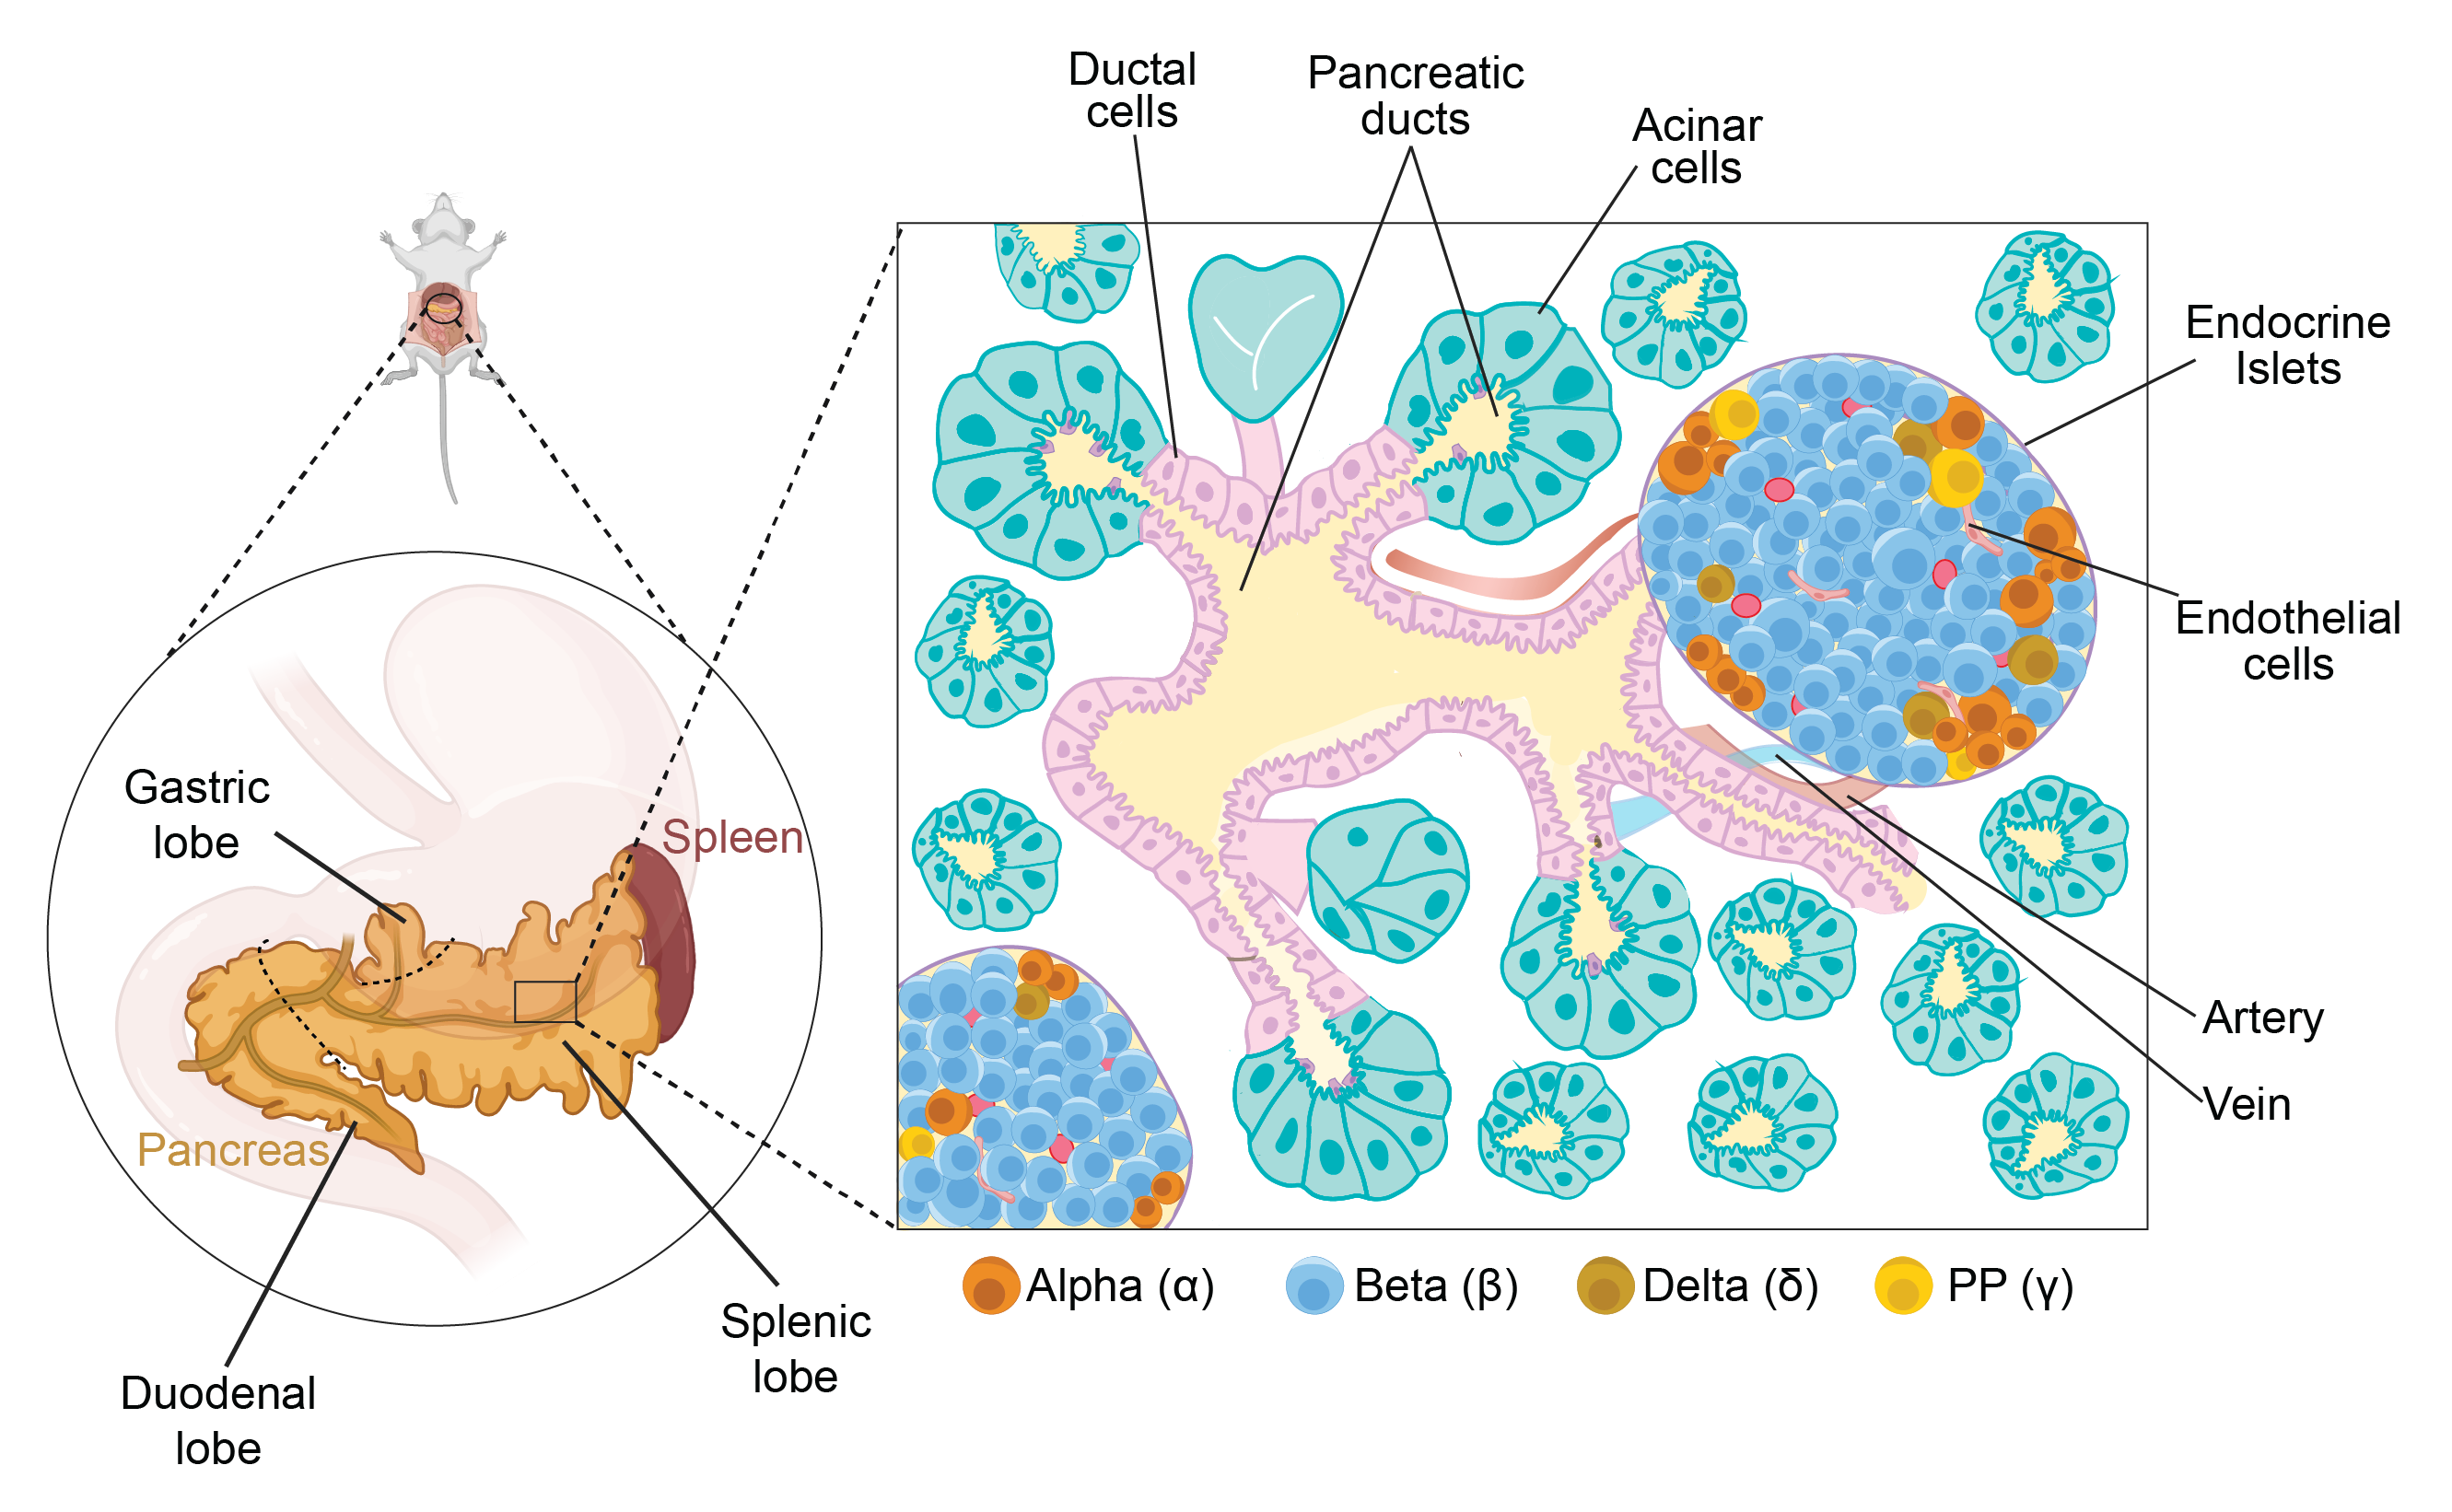
\includegraphics[width=\linewidth]{Chapter1/Fig/F1-1-01.png}
\caption[sec1-1endopanc]{\textbf{Endocrine Pancreas}}
\label{fig1-1}
\end{figure}



The pancreatic tissue in mice is a diffused lobular organ consisting of the duodenal, the splenic, and the gastric lobes. In humans, the pancreas exhibits \st{is} a more compact and well-defined structure, comprising of \st{into three major parts:} the head, the body, and the tail. The pancreas receives a rich vascular supply and the macro-vascular network is conserved in humans and rodents \textbf{\cite{muratore_vascular_2021}}. Although the islets comprise 1-2\% of the pancreas, they receive up to 20\% of the pancreatic blood supply \textbf{\cite{muratore_vascular_2021,jansson_glucose-induced_1986}}. \st{The dense vascularization}This remarkable vascularity of islets is necessary for normal islet function and likely explains how fluctuations in blood glucose are \st{sensed} detected, \st{and lead}leading to rapid and \st{large}substantial changes in the secretion of pancreatic hormones.
\\\\
In rodents such as mice, the islets consist of \textasciitilde75–80\% β-cells, forming a rich “core” and \textasciitilde15–20\% α-cells and the rest is made up by the remaining endocrine cells (δ-cells and PP-cells, <10\% and ε-cells, <1\%), forming the “mantle” of the islet. In contrast, the endocrine cells in the human islets seem to be randomly distributed, and have proportionally fewer β-cells (\textasciitilde55-75\%) and more α-cells (\textasciitilde30-45\%), likely suggesting the major role of glucagon secretion in humans. The variability in cell distribution results in more heterotypic contacts between the endocrine cells in human islets \textbf{\cite{walker_human_2021}}. It has been shown in both mice and humans, that the islet architecture is size-dependent, with smaller islets displaying the core-mantle structure and larger islets with more complex organization \textbf{\cite{dolensek_structural_2015}}. Additional differences in the innervation patterns and presence of smooth muscle cells throughout the vascular network also exist between mouse and human islets \textbf{\cite{rodriguez-diaz_autonomic_2011}}. \st{It is likely that these islet architecture differences between mouse and human}These islet architecture differences between mouse and human likely contribute to physiological differences regarding islet function \textbf{\cite{cabrera_unique_2006}}.
\\\\
To summarize, the pancreatic islets are regarded as a coordinated mini-organ that serves as a remarkable regulator, integrating systemic and local cues to fine-tune blood glucose levels by the synthesis and appropriate secretion of several metabolic hormones by the diverse cell types in the islet microenvironment.

% ********************************** % 1.1.1  **************************************
%\subsection{Principles of (Mendelian) Inheritance} %Section - 1.1.1 
%\label{sec:Mendel}

% ********************************** % 1.1.2 **************************************
% \subsection{Genetic Linkage and the birth of modern genetics} %Section - 1.1.2 
% \label{sec:Morgan}




%%%% Box on genetic terms & origin

%\begin{Comment}
%\hspace{-2.5mm}\textbf{Box 1: Genetic terms \& their origin}\label{box:genetic_terms}
%\small
%\begin{itemize}
%    \item \textbf{Alleles} (originally allelomorphs) were defined by Bateson as the units of inheritance described by Mendel \cite{bateson2013mendel}.
%    \item \textbf{Homozygote} and \textbf{heterozygote} were also used by Bateson to describe individuals carrying the same or different alleles.
%    \item The word \textbf{gene} as a term for the Mendelian factors or units of inheritance was introduced by Danish botanist Johannsen \cite{johannsen1911genotype}. 
%    \item Johannsen also introduced the terms \textbf{phenotype}, as the outward appearance of an individual, and \textbf{genotype}, as their genetic traits. 
%    \item The terms \textbf{polygenetic} (today more often simply polygenic), for traits that are governed by multiple genes, and \textbf{pleiotropic}, for genes that affect multiple, seemingly unrelated, phenotypes also made their first appearance at that time. 
%    \item A \textbf{pedigree}, from the French \textit{pied de grue} (crane's foot), is a diagram that depicts the biological relationships between related individuals.    It is often used to look at the transmission of genetic disorders.
%\end{itemize}
%\vspace{3mm}
%\end{Comment}





% ********************************** % 1.1.3  **************************************
% \subsection{The double helix} %Section - 1.1.3
% \label{sec:double_helix}

% ********************************** % 1.1.4  **************************************
% \subsection{Biometrics} %Section - 1.1.4
% \label{sec:biometrics}

% % %********************************** % 1.1.5  **************************************
% \subsection{Towards quantitative genetics} %Section - 1.1.5
% \label{sec:Fisher}



%\newpage

% % %********************************** % 1.1.6  **************************************
% \subsection{Molecular biology and technological advances}
% \label{sec:genetic_timeline}


% \subsubsection{Cracking the code}
% \label{sec:genetic_code}



% \begin{figure}[htbp]
% \centering
% \includegraphics[width=15cm]{Chapter1/Fig/genetic_timeline_draft.png}
% \caption[Genetic Timeline]{\textbf{150 years of genetics}.\\
% Key scientific discoveries in genetics and corresponding technological advancements.
% A number of scientific discoveries, in combination with key advances in technology and statistical modelling, have led to the identification of thousands of genetic variants which are associated to complex and molecular traits \cite{nhgri2003genetic}.
% Several fundamental contributions have been made, from Mendel's peas to the structure of DNA, to large databases cataloguing genetic variation of hundreds of thousands of individuals.
% Here, I have attempted to highlight the key events that led to today's field of quantitative genetics in the GWAS and post-GWAS era.}
% \label{fig:genetic_timeline}
% \end{figure}

% \subsubsection{Sequencing DNA}
% \label{sec:dna_seq}


% \subsubsection{Understanding the genetic basis of disease}
% \label{sec:disease_genetic}


% \phantomsection
% \label{sec:ld}
% Instead, it was proposed that the combined use of \gls{ld}\footnote{LD: the nonrandom allocation of alleles at nearby variants to individual chromosomes as a result of recent mutation, genetic drift or selection, manifest as correlations between genotypes at closely linked markers \cite{mccarthy2008genome}.} and population- (rather than family-) based studies would be more suitable \cite{risch1996future, jorde2000linkage} - thus practically proposing the design for \glspl{gwas} \cite{risch1996future}.
% However, at the time, implementation of \glspl{gwas} was not possible, for two primary reasons.
% First of all, the technology required to genotype thousands to millions of markers in a single experiment for the larger required sample sizes was not available \cite{risch1996future, visscher2012five}.
% Secondly, the distribution and density of genetic polymorphisms across the genome, and the \gls{ld} between genetic variants across different populations, were unknown.\\

% In some sense, population-based association studies can be viewed as an extension of family-based linkage studies, in which the population studied (derived from common ancestors) acts as an extended pedigree and a much greater number of meiotic recombinations will have occurred between the analysed samples.
% As a consequence, \gls{ld} regions are much smaller than within pedigrees of close relatives, thus requiring a more dense panel of genetic markers to be examined \cite{cordell2005genetic}.

% \subsubsection{The Human Genome Project}
% \phantomsection
% \label{sec:hgp}

% In order to study genomic variation, and therefore its role in disease, it was necessary to generate a reference genome.
% This was the goal of the \gls{hgp}, which aimed at sequencing the entire human genome.
% The \gls{hgp} was 
% % perhaps the first 
% a 
% major breakthrough that dramatically changed the landscape of genetics, and was described by United States President Clinton as “an epic-making triumph of science and reason” \cite{clinton2000remarks} at the announcement of its completion.
% Driven by and a driver of technological breakthroughs in \gls{dna} sequencing and genotyping, the \gls{hgp} was a massive international undertaking and a truly collaborative effort; sequencing and analysis took place across twenty centers in six different countries (USA, UK, France, Germany, Japan, China) and took 13 years to complete, costing approximately \$2.7 billion \cite{lander2011initial}.
% Led in the US by then NIH director Francis Collins and by founder of Celera Genomics\footnote{The company Celera Genomics was formed in May 1998, with the objective of sequencing much of the human genome in three years \cite{venter1998shotgun}.} 
% Craig Venter, and with large contributions from the UK, in particular from the Sanger Institute directed by John Sulston (who had first sequenced the genome of \textit{C. Elegans}), the \gls{hgp} was announced as a joint US-UK statement on June 26th, 2000.
% After a first publication in 2001, the project was truly completed on April 25th, 2003, on the 50$^{th}$ anniversary of the Watson and Crick paper describing the helical structure of \gls{dna}.\\

% The \gls{hgp} provided the first map (obtained from the genomes of a small number of individuals) of the $\sim$3 billion bases in the human genome \cite{lander2001initial, schmutz2004quality, hattori2005finishing}, and revealed that human \gls{dna} consists of surprisingly few exons (1.1\% of the genome), whereas introns cover 24\% of the genome \cite{venter2001sequence, lander2001initial}. 
% Additionally, the number of genes was found to be smaller than expected, with around 30,000 being identified in 2001, and circa 21,000 genes being the latest (still debated) estimate at the time that this thesis is written \cite{pertea2018thousands}. 
% Additional breakthroughs in sequencing technologies have expanded and refined the reference genome, which now captures more than 92\% of the genome and provides a landscape of its genes \cite{lander2011initial}.\\

% With a complete map of the human genome in place, genetic variants could now be identified as those bases discovered in an individual that did not match the (reference) base annotated in the human genome map. 
% Common variants, i.e. variants with \gls{maf}\footnote{The frequency of an
% allele at a genetic locus is the proportion of chromosomes in the study sample that carry that allele \cite{laird2010fundamentals}. 
% For a biallelic variant (a variant for which only two possible alleles are observed in the population), the frequency of the less common (minor) allele is called the minor allele frequency (MAF).} larger than 5\%, were called \glspl{snp}. 
% Previous studies had estimated that approximately 0.1\% (1 base per 1,000) of an individual's genome was a polymorphism \cite{wang1998large, li1991low, cargill1999characterization}. 

% These SNPs were scattered across the genome and it was now time to describe what type of variants they were, where in the genome they were located, and what (if any) effect they had on human phenotypes.

% \subsubsection{The International HapMap Project}

% The International HapMap Project was the first effort of its kind to systematically catalogue genomic variation. 
% Additionally, it aimed to characterise the LD structure of the human genome, which would make GWA studies feasible. 
% The HapMap was officially started in October 2002 as a collaboration between research groups and private companies in Canada, China, Japan, Nigeria, the United Kingdom and the United States with the goal of developing a haplotype map (HapMap) of the human genome \cite{international2003international}.
% By genotyping individuals of African (YRI), European (CEU) and East Asian (JPT, CHB) descent, in Phase I HapMap assembled a publicly available database of common variants (\gls{maf}>5\%) in global samples \cite{international2005haplotype}. 
% The HapMap expanded rapidly. 
% By Phase II (2007), the database contained 2.1 million SNPs from the four original populations \cite{international2007second}.
% Phase III (2010) added genotyping from seven additional populations, for a total of over 3 million SNPs in 11 global ancestry groups\footnote{ASW (African ancestry in Southwest USA); CEU (Utah residents with Northern and Western European ancestry from the CEPH collection); CHB (Han Chinese in Beijing, China); CHD (Chinese in Metropolitan Denver, Colorado); GIH (Gujarati Indians in Houston, Texas); JPT (Japanese in Tokyo, Japan); LWK (Luhya in Webuye, Kenya); MEX (Mexican ancestry in Los Angeles, California); MKK (Maasai in Kinyawa, Kenya); TSI (Tuscans in Italy); YRI (Yoruba in Ibadan, Nigeria).} \cite{international2010integrating}.\\ 

% The growing popularity of genetic association studies in parallel with the expansion of the HapMap effort paved the way for the last needed technological breakthrough: microarrays.
% By knowing the genetic location of thousands of variants, commercial companies were able to develop so-called `SNP chips' \cite{meaburn2006genotyping, oliphant2002beadarray}, which allowed for genotyping at specific locations across the genome.
% In parallel, the data generated by the HapMap project enabled calculation of the LD\footnote{Pearson's correlation coefficient squared, $r^2$, is commonly used} between SNPs within the genome, effectively describing the chance that two SNPs will be inherited together \cite{bush2012genome}.
% This enabled the identification of haplotypes and thus a minimal set of SNPs that capture the majority of the haplotype diversity within a population, called `tag SNPs' \cite{international2003international}. 
% The collective LD information gathered by academics in those years \cite{slatkin2008linkage, pe2006evaluating, otto2002resolving} allowed companies such as Affymetrix and Illumina to develop SNP arrays that contained 
% these tag SNPs, effectively capturing information about common variation across a large percentage of the genome while only directly genotyping a few thousand SNPs.\\

%\newpage

% % %********************************** % 1.1.7  **************************************
% \subsection{Genome-wide association studies}
% \label{sec:gwas}

% The data generated by the International HapMap Project combined with development of appropriate chip-based microarray technology, which enabled simultaneous genotyping of more than one million SNPs, led to the first wave of \glspl{gwas} \cite{visscher2012five}.
% \gls{gwas} are a hypothesis-free\footnote{bar the selection of SNPs on the chip. 
% More recently, shallow DNA-seq has been increasingly used as an alternative, making the approach truly hypothesis-free.} approach to test for statistical association between the genotype frequency of common genetic variants (considered one by one across the genome) and a phenotype of interest \cite{mccarthy2008genome}. 
% The development of GWAS was accompanied by great enthusiasm, and the hope that these studies could better our understanding of the genetic underpinning of human disease, leading to improvement of prognosis and acceleration of drug and diagnostics development. \\

% Initially, \gls{gwas} focused on complex phenotypes with binary outcomes, using a case-control design (i.e. diseased vs healthy).
% Then, for each SNP and binary trait, the association was evaluated using a Cochran–Armitage (trend) test, a $\chi^2$ test or a Fisher's exact test comparing the numbers of cases and controls when stratified by their alleles at the locus of interest. 
% The first successful \gls{gwas} was published in 2002 on myocardial infarction \cite{ozaki2002functional}.
% The same design was then applied in a landmark GWA study conducted in 2005 for age-related macular degeneration (AMD), using 96 cases and 50 healthy controls and testing for associations at $\sim$100,000 SNPs \cite{klein2005complement}. 
% In 2007, the Wellcome Trust Case-Control Consortium (WTCCC) published a study where they performed \gls{gwas} on seven different common diseases, using 2,000 cases for each of bipolar disorder (BD), coronary artery disease (CAD), Crohn's disease (CD), hypertension (HT), rheumatoid arthritis (RA), type I and II diabetes (T1D, T2D) and a common set of 3,000 healthy controls, demonstrating the feasibility of the use of a shared set of controls across several traits \cite{wellcome2007genome}.\\

% A year later, in 2008, the \gls{gwas} Catalog was founded to keep a record of all published \gls{gwas} and identified associations \cite{welter2014nhgri}.
% As of September 2020, when I am writing this thesis, the \gls{gwas} Catalog includes 4,694 publications, describing 197,708 SNP-trait associations \cite{macarthur2017new}.\\

% Over time, quantitative traits have become increasingly popular to use as phenotypes, in addition to binary traits.
% These include continuous traits such as height, weight and blood pressure.
% Furthermore, linear regressions and their derivations have become more popular methods to assess association, due to their flexibility to include covariates \cite{mccarthy2008genome}.
% I describe these models in detail in the next chapter (\textbf{Chapter \ref{chapter2}}). 

%\newpage

% \gls{gwas} results are often visualised using a Manhattan plot \cite{mccarthy2008genome}, where the negative log p value (as a measure of significance) is plotted on the y axis, against the corresponding genomic position (ordered by chromosome and position) on the x axis (\textbf{Fig. \ref{fig:manhattan}}). 
% Peaks on these plots represent loci (multiple variants in \gls{ld}) that display evidence of association with the analysed phenotype. 
% Variants are deemed to be significantly associated with a trait if they exceed an appropriately chosen p value threshold. 

%\begin{figure}[h]
%\centering
%\includegraphics[width=15cm]{Chapter1/Fig/Manhattan_plots_CD_WTCCC_2007.jpg}
%\caption[Manhattan plot]{\textbf{Manhattan plot}.\\
%Manhattan plot for Crohn's disease (CD) from the WTCCC study \cite{wellcome2007genome}.
%On the x axis are plotted the genomic positions of the SNPs tested, one chromosome after %the next.
%On the y axis are the association significance values.  
%Alternating colours are used to distinguish chromosomes (odd numbered chromosomes -and chromosome X- are dark, even numbered chromosomes are light).
%Highlighted in green are statistically significant SNPs (p value < $5 \times 10^{-8}$).}
%\label{fig:manhattan}
%\end{figure}

%\subsubsection{From global traits to molecular traits}

 

% % %********************************** % 1.1.8  **************************************
% \subsection{Expression quantitative trait loci}
% \label{sec:eqtl}

% \subsubsection{Mechanisms of the genetic regulation of gene expression}


% \subsubsection{Mapping eQTL}
% \label{sec:eqtl_map}

 
 
% \subsubsection{\textit{Cis} and \textit{trans} eQTL}



% \begin{figure}[h]
% \centering
% \includegraphics[width=15cm]{Chapter1/Fig/eqtl.png}
% \caption[\textit{Cis} and \textit{trans} eQTL]{\textbf{\textit{Cis} and \textit{trans} eQTL}.\\
% \textit{Cis} eQTL affect the expression of genes directly. 
% \textit{Trans} eQTL, in contrast, affect the expression of typically more distant genes, often by first having a \textit{cis} effect on the expression of intermediate regulatory genes.
% % On the right, the typical representation of eQTL using box plots.
% Figure adapted from \cite{westra2014genome}.
% }
% \label{fig:eqtl}
% \end{figure}



% \subsubsection{From tissue-specific to cell type-specific eQTL}
% \label{sec:eqtl_celltype_specific}



% \subsubsection{Context-specific eQTL}


% \newpage

% \subsubsection{Using eQTL to link genes to disease}
% \phantomsection
% \label{sec:eqtl_gwas}



% \subsubsection{eQTL mapping in iPSC and iPSC-derived cells}



% ***********************************************************************************************************************************************************************************************************************************************************************************************************************************

\newpage

% \vspace*{10px}

% \textit{“It is not birth, marriage, or death, but gastrulation which is truly the most important time in your life.”}\\
% \rightline{Lewis Wolpert, 1986}

% \vspace*{5px}

% ***************************************************************
%************************ %Second Section %****************************************************************
\section{ Islet \( \mathbf{\upbeta} \)-cells}  %Section - 1.2
\label{sec:human_ipscs}  

% ********************************** % 1.2.1  **************************************
\subsection{Pancreas Organogenesis} %Section - 1.2.1 
\label{sec:pancorgano}

Pancreas organogenesis is a \st{highly} conserved process during fetal development and comprises a tightly coordinated and regulated interplay of complex signaling events. During this step-wise program, the pancreas develops from a simple bud-like structure to a \st{final} mature, highly branched organ containing several specialized cell types. In mice, the pancreas specification begins at embryonic day 8.5 \textbf{(e8.5)} with the formation of dorsal and ventral pre-pancreatic regions in the foregut endoderm \textbf{\cite{shih_pancreas_2013, slack_developmental_1995}}. The pancreas development becomes morphologically evident at  \textbf{\textasciitilde e9.5} when the presumptive pancreatic regions in the endoderm undergo thickening and eventually result in the emergence of pancreatic buds \textbf{\cite{shih_pancreas_2013}}. Over the next 2-3 days, the pancreatic buds continue to elongate, accompanied by the stratification of the epithelium and the formation of multiple micro-lumens \textbf{\cite{pan_pancreas_2011}}. At \textbf{\textasciitilde e12.5}, as a result of both due to gut rotation and elongation of the dorsal and ventral stalks, the pancreatic buds (dorsal and ventral) come into contact and fuse into a single organ. \textbf{This early phase of pancreatic development is referred to as the “primary transition”.}
\\\\

% ********************************** % 1.2.2  **************************************
\subsection{Endocrine Cell Development} %Section - 1.2.2 
\label{sec:endodev}
The vast majority of the endocrine cells arise during the secondary transition from the endocrine progenitors \textbf{\cite{pan_pancreas_2011}}. However, glucagon-containing α-cells can be seen as early as \textbf{e9} in the primordium \textbf{\cite{pictet_ultrastructural_1972,gittes_developmental_2009}}. The fate decision in the bi-potent trunk domain during the secondary transition is determined by graded \textit{Notch} activity. Lower \textit{Notch} activity leads to \textit{Sox9} expression, which is an activator of \textit{Ngn3} \textbf{\cite{shih_pancreas_2013}}, a basic-helix-loop-helix \textbf{(bHLH)} transcription factor \textbf{(TF)} and master regulator of endocrinogenesis \textbf{\cite{gu_direct_2002}}. Cells that do not escape \textit{Notch} signaling express both \textit{Hes1} and \textit{Sox9}, resulting in \textit{Ngn3} repression and eventual contribution to the ductal tree. \st{However, no signals have yet been identified that could account such a segregated expression pattern of Ngn3.} After \textit{Ngn3} expression, endocrine progenitors exit the cell-cycle and delaminate into surrounding stromal tissue \textbf{\cite{shih_pancreas_2013, gouzi_neurogenin3_2011, miyatsuka_neurogenin3_2011}}. These \textit{Ngn3+} cells are uni-potent and as a whole can generate the five different endocrine cell types \textbf{\cite{shih_pancreas_2013,gu_direct_2002,miyatsuka_neurogenin3_2011}}. The timing and strength of \textit{Ngn3} expression determines the efficiency of endocrine cell formation and the cell type: early \textit{Ngn3} expression results in formation of α-cells while delayed expression of \textit{Ngn3}  generates β- and δ-cells followed by γ-cells\textbf{\cite{johansson_temporal_2007}}.
\\\\
Critical TFs such as \textit{Pax4}, \textit{Pdx1} and \textit{Nkx6.1} control the determination of β-cell fate. On the contrary, \textit{Arx} determines α-cell identity. Both \textit{Pax4} and \textit{Arx} are targets of \textit{Ngn3} and are co-expressed, after which they begin to repress each other. In the \textit{Nkx6.1+} β-cell precursors, the switch from the TF \textit{MafB} \st{(v-Maf avian musculoaponeurotic oncogene homolog B)} to \textit{MafA} expression is an important step to activate the complete the β-cell specific program. After birth, immature β-cells undergo stepwise maturation to become fully mature cells.
\\\\
% ********************************** % 1.2.3  **************************************
\subsection{Postnatal \( \mathbf{\upbeta} \)-cell maturation} %Section - 1.2.3
\label{sec:betamat}
β-cell maturation is continuation of β-cell development and occurs postnatally in mammals (https://link.springer.com/article/10.1007/s00125-022-05672-y). Most of the current understanding of β-cell maturation process is derived from neonatal rodent islets, as similar data from humans is difficult to collect \textbf{\cite{liu_all_2017, salinno_-cell_2019}}. After birth, immature β-cells undergo several steps to become fully mature and functional cells characterized by tightly controlled insulin secretion in response to glucose.
\\\\
The immature β-cells are organized into clusters, forming proto-islets \textbf{\cite{salinno_-cell_2019}}, which eventually undergo structural rearrangements to form the compacted core and mantle architecture \textbf{\cite{sharon_peninsular_2019}}. The developmentally immature β-cells are characterized by a strong proliferative capacity, thereby resulting in a general increase in β-cell mass. The immature β-cells present insulin granules but display “leaky” insulin secretion wherein they have a decreased glucose threshold for stimulated insulin secretion \textbf{\cite{liu_all_2017, blum_functional_2012}} and are less glucose-responsive thereby affecting their ability to regulate insulin secretion in response to fluctuating blood glucose levels. \st{[ref]. <continue from PAI>}
\\\\
Immature β-cells follow a biphasic pattern of maturation \textbf{\cite{salinno_-cell_2019, stolovich-rain_weaning_2015}}.  The first wave starts right after birth and lasts until \textasciitilde 2 weeks, during which β-cells increase the expression of several key TFs and associated machinery necessary to establish adult β-cell identity. Some of the key signature genes include \textit{Pdx1}, \textit{Neurod1}, \textit{Nkx2.2} and \textit{Nkx6.1}, which are expressed by all β-cells at birth \textbf{\cite{salinno_-cell_2019}}. In addition, several other markers have also been identified which mark the early phase of functional maturation of β-cells: increased expression of \textit{Ucn3} \textbf{\cite{salinno_-cell_2019, blum_functional_2012}}, \textit{Syt4} \textbf{\cite{salinno_-cell_2019, huang_synaptotagmin_2018}}, \textit{Fltp} \textbf{\cite{salinno_-cell_2019, bader_identification_2016}}  and dramatic drop in levels of \textit{Npy} \textbf{\cite{salinno_-cell_2019, rodnoi_neuropeptide_2017}}. Among TFs, \textit{MafA} progressively substitutes \textit{MafB} expression and further regulates expression of genes involved in glucose sensing and insulin secretion, thereby characterizing the late phase of postnatal maturation.
\\\\
The second wave of maturation occurs from about the third week of life until the weaning period involving dietary change from high-fat maternal milk to a high-carbohydrate chow diet. During this weaning phase, β-cells begin to exhibit improved glucose-stimulated insulin secretion and glucose-induced replication, although the latter remains to be explained. This phase is characterized by β-cells differentially regulating metabolic pathways, involving a switch from mTORC1 to AMPK-dependent signaling, which defines the mature functional landscape. The dietary change associated with the weaning period also affects the secretion of incretin hormones, which enhance GSIS and modulate β-cell replication.
\\\\
% ********************************** % 1.2.4  **************************************
\subsection{Insulin Biosynthesis} %Section - 1.2.4
\label{sec:insbio}
Blah blah blah
\\\\
% ********************************** % 1.2.5  **************************************
\subsection{Glucose-Stimulated Insulin Secretion (GSIS)} %Section - 1.2.5
\label{sec:gsis}
blah blah blah
\\\\
% ********************************** % 1.2.6  **************************************
\subsection{Regulation of GSIS} %Section - 1.2.6
\label{sec:reggsis}
blah blah blah
\\\\
% ********************************** % 1.2.7  **************************************
\subsection{Insulin Action and Clearance} %Section - 1.2.7
\label{sec:insact}
Insulin exerts its known physiological effects by binding to the insulin receptor (InsR) on the surface of target cells. The InsR assembles as a tetramer, consisting of two extracellular alpha subunit, which binds insulin and a two membrane-spanning beta subunit, with a tyrosine-kinase domain each. The activation of this kinase results in a metabolic signaling cascade downstream, eventually leading to the uptake of glucose, lipids and amino acids into the cells. The two principal pathways resulting from this interaction include the phosphoinositide 3-kinase (PI3K)/Akt pathway and the Ras/mitogen-activated protein kinase (MAPK) pathway. The PI3K/Akt pathway is critical for linking insulin receptor substrate (IRS) proteins to the metabolic actions of insulin whereas the Ras/MAPK pathway is primarily associated with the growth and mitogenic effects of insulin \textbf{\cite{de_meyts_insulin_2000}}. The binding of insulin to InsR in the target tissues stimulates the translocation of glucose transporter 4 (GLUT4) storage vesicles from intracellular pools to the cell surface, thereby increasing the rate of glucose uptake \textbf{\cite{shepherd_glucose_1999,saltiel_insulin_2001,leto_regulation_2012}}. In the absence of insulin, only ~5\% of GLUT4 pool can be found on the plasma membrane \textbf{\cite{leto_regulation_2012}}.
\\\\


% %********************************** % 1.2.1  **************************************
% \newpage

% \subsection{From homunculi to developmental biology}
% \label{sec:history_developmental_biology}



% \begin{wrapfigure}{r}{0.6\textwidth}
% \includegraphics[width=9.5cm]{Chapter1/Fig/Early_theories_development.png}
% \caption[Early theories of development]{\textbf{Early theories of development}.\\
% Illustration of the two leading theories on human embryology before the 19$^{th}$ century.
% Left, Illustration of Preformation: 
% A tiny person (homunculus) growing inside a sperm, as drawn by Nicolaas Hartsoeker in 1695.
% Right, Epigenesis: study of foetus deveopment by Leonardo Da Vinci, c. 1510.}
% \label{fig:early_embryology}
% \end{wrapfigure}




\newpage

% \subsection{}}
% \label{sec:human_embryogenesis}




% \begin{figure}[h]
% \centering
% \includegraphics[width=14.5cm]{Chapter1/Fig/embryogenesis_til_gastrulation.png}
% \caption[Human Embryogenesis]{\textbf{Human Embryogenesis}.\\
% Early stages of human embryogenesis.
% (a) From zygote to morula: stages of clevage.
% (b) The blastocyst.
% Cells divide and form an outer layer, the trophoblasts.
% Inner cells also called embryoblasts get compacted and move to a side forming the inner cell mass (ICM), leaving a fluid filled cavity called the blastocoel.
% (c) The formation of the bilaminar disk.
% The ICM splits into the epiblast and hypoblast which distribute along the surface and result into two more cavities, the amniotic cavity and the primitive yolk sac, respectively.
% (d) Gastrulation: from bilaminar to trilaminar disk.
% The primitive streak forms and cells start to migrate moving down in between the epiblast and the hypoblast.
% The endoderm, mesoderm and ectoderm form and are called the trilaminar disk.}
% \label{fig:embryogenesis}
% \end{figure}

 

% \subsection{Human Stem Cells}
% \label{sec:escs} 


% \begin{figure}[htbp]
% \centering
% \includegraphics[width=16cm]{Chapter1/Fig/stem_cell_potency.png}
% \caption[Stem Cells]{\textbf{The potency tree of stem cells}.\\
% The spectrum of potency along human development: from the totipotent zygote to terminally differentiated cells.}
% \label{fig:stem_cells}
% \end{figure}

% \subsubsection{Embryonic stem cells}
% \label{sec:esc_induction}




% %********************************** % 1.2.3  **************************************
% \subsection{Nuclear cloning of somatic cells}
% \label{sec:cloning} 


% %********************************** % 1.2.1  **************************************
% \subsection{Induced pluripotent stem cells}
% \label{sec:ipsc}
   

%\begin{figure}[h]
%\centering
%\includegraphics[width=15cm]{Chapter1/Fig%/ipsc_timeline.png}
%\caption[iPSCs timeline]{\textbf{Historical timeline of key events leading to the development of iPS cells}.\\
%Key events including somatic cloning and isolation of ES cells that eventually led Shinya Yamanaka and colleagues to generate iPSCs in 2006 and Yamanaka to win the 2012 Nobel Prize for Physiology and Medicine alongside Sir John Gurdon.}
%\label{fig:ipsc_timeline}
%\end{figure}

% \newpage

% \subsubsection{Inducing pluripotency}

% \subsubsection{Challenges in the use of iPSCs}
% \subsubsection{Reprogramming factors}
% \subsubsection{Mechanisms of iPSC induction}



%\begin{figure}[htbp]
%\centering
%\includegraphics[width=14cm]{Chapter1/Fig/ipscs.png}
%\caption[iPS cells]{\textbf{iPS cells - derivation and applications}.\\
%The generation of iPSCs starts with a biopsy from, for example, the skin of an adult donor.
%Adult cells, in the example fibroblasts, are then isolated and pluripotency is induced through four reprogramming factors, for example the Yamanaka factors: Oct4, Sox2, Klf4 and c-Myc (OSKM).
%The factors can be delivered using a number of systems, see \textbf{page \pageref{sec:ipsc_delivery}}.
%The resulting induced pluripotent stem cells (iPSCs) are self-renewing and are virtually indistinguishable from ESCs.
%They can be subsequently differentiated towards other cell types, including disease relevant cell types, for example dopaminergic neurons for Parkinson's disease, or pancreatic beta cells for diabetes.
%In the future, iPSC-derived cells might be used for cell therapy, i.e. they could be transplanted into the patient, with no risk of allogenic rejection.
%In the meantime, iPSCs and iPSC-derived differentiations can be used to model development and disease, and to do compound screening and drug testing.
%Figure created with BioRender.com.}
%%\label{fig:ipsc}
%\end{figure}


% \subsubsection{Delivery methods}
% \label{sec:ipsc_delivery}




% \subsubsection{Somatic cell of origin}
% \label{sec:ipsc_somatic_cell}



% \subsubsection{Characterising iPSCs}
% \label{sec:ipsc_characterise}



% \subsubsection{Heterogeneity of iPSCs and between cell line variation}


% \subsection{Applications of human iPSCs in genetics}
% \label{sec:ips_genetics}





% \subsubsection{HipSci and other human iPSC consortia}
% \label{sec:HipSci}


% \subsubsection{eQTL mapping using iPSCs and iPSC-derived cells}


% \newpage

% %********************************** %Third Section  **************************************
\section{Diabetes Mellitus}


Diabetes Mellitus (DM), commonly referred to as diabetes, is a group of complex metabolic disorders that has reached pandemic proportions, and poses a significant global health challenge. \st{As of 2019, approximately 463 million adults aged 20-79 were diabetic and this number is projected to rise to ~700-800 million by 2045.} The International Diabetes Federation (IDF) reported that 10.5\% of the adult population (20-79 years) had diabetes in 2021, and projected that this proportion would increase to 13.7\% by 2045 \cite{home_idf_nodate}. In Germany, an estimated 7\% of the adult population was diabetic in the year 2021 \cite{noauthor_germany_nodate}. Diabetes is associated with several long-term complications such as kidney failure, cardiovascular diseases and is a major risk factor for blindness, lower limb amputation, \st{stroke}and stroke and nerve damage \cite{ashcroft_diabetes_2012,emerging_risk_factors_collaboration_diabetes_2010,leon_diabetes_2015}. Consequently, diabetes stands as one of the foremost causes of global mortality \st{Altogether, this makes diabetes a leading cause of mortality worldwide} with 6.7 million deaths in 2021 \cite{home_idf_nodate}. These premature deaths and comorbidities \st{due to diabetes} inflict a huge economic strain on healthcare systems. The IDF estimated an expenditure of at least USD 966 billion in diabetes related causes in 2021 \cite{home_idf_nodate}. To address this burgeoning crisis and mitigate risk factors a multifaceted approach is essential with research efforts directed towards unraveling the complex interplay of genetic, environmental, and lifestyle factors that contribute to the development of diabetes. 

% ********************************** % 1.3.1  **************************************
\subsection{Forms of Diabetes} %Section - 1.3.1 
\label{sec:forsmDiabets}

DM \st{Diabetes mellitus (short - diabetes)} is \st{a group of complex metabolic disorders} characterized by sustained high blood glucose concentrations (hyperglycemia) \st{because of insufficient supply of insulin} resulting from inadequate insulin production, impaired insulin action, or a combination of both. Diabetes is broadly classified into two main types: Type 1 and Type 2  The current classification relies both disease etiology and pathogenesis \textbf{\cite{banday_pathophysiology_2020}}, serving as a valuable tool in clinical disease assessment and therapy determination. Based on this, diabetes can be divided into four main categories:\\
\begin{enumerate}
    \item Type 1 DM \textbf{(T1DM)}
    \item Type 2 DM \textbf{(T2DM)} 
    \item Gestational DM \textbf{(GDM)} and 
    \item Diabetes associated with certain specific conditions and/or disorders.
\end{enumerate}


%\begin{figure}[htbp]
\begin{figure}[t]
\centering
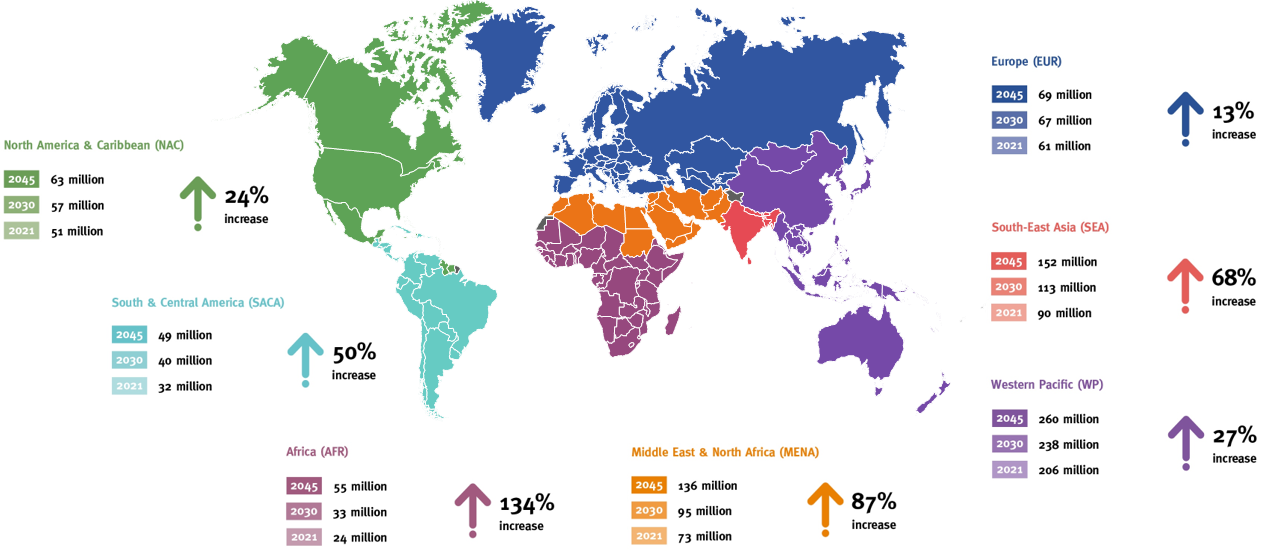
\includegraphics[width=14cm]{Chapter1/Fig/IDF.png}
\caption[diabetes]{\textbf{IDF Atlas 2021}.\\\\
The generation of iPSCs starts with a biopsy from, for example, the skin of an adult donor.
Adult cells, in the example fibroblasts, are then isolated and pluripotency is induced through four reprogramming factors, for example the Yamanaka factors: Oct4, Sox2, Klf4 and c-Myc (OSKM).}
%\label{fig:ipsc}
\end{figure}

\subsubsection{T1DM}

Type 1 DM (T1DM) is a chronic, autoimmune disorder in which the insulin-secreting \textbeta-cells are progressively lost, and immune cell infiltration into the pancreatic islets play a crucial role in this process. The destruction of \textbeta-cells, caused by auto-reactive CD4 and CD8 T-cells results in little to no insulin production causing hyperglycaemia. As the disease progresses, auto-antibodies targeting \textbeta-cell proteins, especially native insulin, manifest and are subsequently joined by auto-antibodies against other proteins (glutamic acid decarboxylase or zinc transporter 8), leading to an expansion of auto-reactivity and eventual development of overt clinical disease (marked by destruction of 85-90\% of \textbeta-cells).
\\\\
T1DM is typically presents during diagnosed in childhood and adolescence,\st{but not exclusively, and accounts for 5-10\% of all cases of diabetes} although it can occur at any age, contributing to 5-10\% of all diabetes cases \textbf{\cite{banday_pathophysiology_2020}}. The etiology of T1DM is multifactorial, involving both, genetic predisposition and environmental triggers \st{play an important role in in its the pathogenesis. of T1DM}. The current therapeutic strategy entails daily exogenous administration of insulin to maintain stable glucose levels. Alternative approaches include a hybrid-closed loop model (artificial pancreas) for regulated insulin delivery, primary islet transplantation or immuno-modulation, albeit, the latter two present their own set of challenges. Additionally, early clinical trials involving stem cell therapies, such as mesenchymal stem cell (MSC) therapy have shown promising results as potential treatments for T1DM \textbf{\cite{pathak_therapies_2019}}.

\subsubsection{T2DM}

Type 2 DM (T2DM) develops from high insulin demand due to insulin resistance in peripheral target tissues. The insulin resistant state manifests several years prior to T2DM diagnosis. Functional β-cells can match the increased metabolic demand by secreting more insulin in order to maintain normal glucose levels. However, sustained demand over chronic periods leads to progressive β-cell dysfunction, resulting in glucose intolerance and overt disease. \textbf{Insulin resistance and β-cell dysfunction are considered as major hallmarks of T2DM \cite{banday_pathophysiology_2020}}. 
\\\\
While, genome-wide association studies (GWAS) have been able to identify the genetic susceptibility to T2D \textbf{\cite{grarup_genetic_2014, wang_genetic_2016}}, other factors, particularly obesity have demonstrated a strong link to insulin resistance and T2DM pathogenesis. Excessive obesity causes a metabolic overload of the adipose tissue, resulting in chronic inflammation via secretion of pro-inflammatory cytokines such as TNF-a, IL-6, IL-1B and MCP-1 \textbf{\cite{guilherme_adipocyte_2008}}. The macrophages recruited into the adipose tissue create a chronically inflamed state and reduce the uptake of fatty acids by skeletal muscle. The elevated levels of these free fatty acids impair signaling and insulin-stimulated glucose transport leading to the development of insulin resistance \textbf{\cite{unger_lipotoxicity_1995,uysal_protection_1997,kanda_mcp-1_2006}}. However, the critical determinant for T2D is β-cell dysfunction \textbf{\cite{tahrani_glycaemic_2010, khin_pancreatic_2023}}, which is more severe than insulin resistance. The interplay between β-cell dysfunction and insulin resistance is highly complex; however, they likely influence each other and synergistically worsen T2DM.  Several factors are thought to contribute to β-cell dysfunction – chronic nutrient overload (glucotoxicity and glucolipotoxicity) \textbf{\cite{prentki_nutrient-induced_2020}}, insulin secretory defects \textbf{\cite{kahn_mechanisms_2006}}, reduced β-cell mass, amyloid deposition \textbf{\cite{prentki_islet_2006}} and/or islet inflammation and oxidative stresses. \st{The role of islet inflammation in T2D and its involvement in β-cell dysfunction is discussed at length in Chapter 2.}
\\\\
T2DM accounts for 90-95\% of all diagnosed diabetic cases53,57,70. Due to the multi-faceted and progressive nature, the treatment for T2D follows a step-wise approach. The very first recommended therapeutic intervention is the adoption of a healthier life style: more healthy diet, increased physical activity and maintaining a healthy body weight. The first anti-diabetic drug to be usually prescribed is Metformin, which works by reducing hepatic gluconeogenesis, delaying intestinal absorption and improving the overall insulin sensitivity71, although accumulating evidence points to possible new mechanisms of actions72. The persistence of T2DM further requires a additional medications as monotherapy is insufficient to maintain normal blood glucose levels53,73. Other available anti-diabetic drugs include sulphonylureas, glucagon-like peptide 1 (GLP-1) agonists, thiazolidinediones, sodium-glucose cotransporter 2 (SGLT2) inhibitors or dipeptidyl peptidase 4 (DPP-4) inhibitors 53,73,74. Upon failure of these antidiabetic drugs, intensive insulin therapy via exogenous administration becomes necessary in order to maintain the target range of blood glucose levels in T2DM patients and avoid health complications 53.
\\\\
T1DM and T2DM together account for most of the diabetes cases. Besides these two, there are also less common forms of diabetes:


%The overall aim of this thesis is to provide suitable computational methods for the identification of cell type and context-specific eQTL using single cell expression profiles, and explore their application across a range of human iPSC-derived cell types, using data from the \gls{hipsci} project.\\

%Specifically, in \textbf{Chapter \ref{chapter2}}, I provide an overview of the use of linear and \glspl{lmm} for genetic association analyses, focusing on their application in \gls{eqtl} mapping.\\

%In \textbf{Chapter \ref{chapter3}}, I describe best-practice approaches to perform \gls{eqtl} mapping using \gls{scrnaseq} profiles and demonstrate these methods on matched bulk and single cell expression of around 100 human \gls{ipsc} lines. \\

%In \textbf{Chapter \ref{chapter4}}, I present a dataset of almost 40,000 cells from 125 human \gls{ipsc} lines differentiating to definitive endoderm, and demonstrate different approaches to \gls{eqtl} mapping using \gls{scrnaseq} data, identifying genetic variants that affect gene expression dynamically along differentiation and across other cellular states. \\

%In \textbf{Chapter \ref{chapter5}}, I present a dataset of over one million cells from 215 human \gls{ipsc} lines differentiating to midbrain dopaminergic neurons. We identify thousands of \glspl{eqtl} across a number of cell types and upon external stimulation. In addition, we identify hundreds of colocalisation events with variants that are known to be associated with neurological traits and diseases. Moreover, we investigate sources of variation in the capacity of individual cell lines to differentiate toward neurons.\\

%Finally, in \textbf{Chapter \ref{chapter6}}, I conclude and discuss future directions.
\newpage

% ***************************************************************
%************************ %Fourth Section %****************************************************************
\section{scRNA-seq}  %Section - 1.4
\label{sec:scrna} 

\subsection{Introduction}
\label{sec:141}


\subsection{Other Modalities}
\label{sec:142}

Besides single-cell transcriptomics, a range of other technologies aims to profile the distinct layers contributing to the overall molecular make-up of a cell. Collectively, these single-cell methodologies enable us to uncover cellular diversity from novel perspectives, offering comprehensive and impartial analyses of individual cells 126. Some of these modalities are:

